\chapter{Arithmetic Foundations}\label{sec:arithmetik}

In this chapter we investigate the number-theoretic properties of the
sequence~\eqref{eq:k_main} and derive the structure of its differences.

\section{Derivation via Means of Sums of Squares}

The sequence $k(n)$ arises naturally from the classical summation formula
for square numbers. For the sum of the first $n$ squares one has
\begin{equation}\label{eq:quadratsumme}
S_n = \sum_{i=1}^{n} i^2 = \frac{n(n+1)(2n+1)}{6}.
\end{equation}

The arithmetic mean of these squares is
\begin{equation}
M_n = \frac{S_n}{n} = \frac{(n+1)(2n+1)}{6} = \frac{2n^2 + 3n + 1}{6} = k(n).
\end{equation}

\begin{remark}
The sequence $k(n)$ thus gives the \emph{average value} of the first $n$
square numbers. It is the parabolic interpolation form of the arithmetic mean.
This interpretation is important for understanding the later geometric
construction, as it establishes the connection between discrete summation
and continuous geometry.
\end{remark}

The following table illustrates the structure of the sums of squares and
their means for the first fifteen values:

\begin{center}
\begin{tabularx}{\textwidth}{c|S[table-format=1.0]*{14}{>{\raggedleft\arraybackslash}X}} 
\toprule
$n$ & \textbf{1}& 2 & 3 & 4 & \textbf{5} & 6 & \textbf{7} & 8 & 9 & 10 & \textbf{11} & 12 & \textbf{13} & 14 & 15 \\
\midrule
$n^{2}$ & 1& 4 & 9 & 16 & 25 & 36 & 49 & 64 & 81 & 100 & 121 & 144 & 169 & 196 & 225 \\
\midrule
$\smash{\textstyle\sum_{k=1}^{n} k^2}$ & 1& 5 & 14 & 30 & 55 & 91 & 140 & 204 & 285 & 385 & 506 & 650 & 819 & 1015 & 1240 \\
\midrule
$M_n$ & \textbf{1} & {\scriptsize 2.5} & {\scriptsize $4.\overline{6}$} & {\scriptsize 7.5} & \textbf{11} & {\scriptsize $15.1\overline{6}$} & \textbf{20} & {\scriptsize 25.5} & {\scriptsize $31.\overline{6}$} & {\scriptsize 38.5} & \textbf{46} & {\scriptsize $54.1\overline{6}$} & \textbf{63} & {\scriptsize 72.5} & {\scriptsize $82.\overline{6}$} \\
\bottomrule
\end{tabularx}
\end{center}

The bold values indicate the integer means, which occur precisely for
$n \equiv 1, 5 \pmod{6}$.

\begin{remark}[Connection to the OEIS: A164576]
	The sequence of integer means
	\[
	1,\; 11,\; 20,\; 46,\; 63,\; 105,\; 130,\; 188,\;\ldots
	\]
	is listed in the OEIS under \href{https://oeis.org/A164576}{A164576}~\cite{OEIS}
	as \emph{``Integer averages of the set of the first positive
		squares up to some $n^2$''} --- precisely the sequence $k(n)$ whose
	discovery stands at the beginning of this work.
	
	The OEIS formula (Colin Barker, 2015) reads:
	\[
	a(j) = \frac{1}{4}\bigl(12j^2 - 6j + (-1)^j(4j-1) + 1\bigr),
	\qquad j = 1, 2, 3, \ldots
	\]
	It uses a \emph{running} index $j$ that enumerates the integer
	positions $n \equiv 1, 5 \pmod{6}$ consecutively.
	The factor $(-1)^j$ is a \emph{quasi-polynomial of period~$2$}:
	it encodes both congruence classes in a single expression --- for
	odd $j$ (i.e.\ $n \equiv 1 \pmod{6}$) and even $j$
	(i.e.\ $n \equiv 5 \pmod{6}$) it alternately takes the values
	$+1$ and $-1$.
	
	The connection to $k(n)$ is obtained by substituting
	$A007310(j)$ --- the sequence of positive integers coprime
	to~$6$~\cite{OEIS}:
	\[
	a(j) = k\!\bigl(A007310(j)\bigr),
	\]
	where the two branches yield precisely:
	\[
	k(A007310(j)) =
	\begin{cases}
		\dfrac{(2j-1)(3j-1)}{2} & j \text{ odd } (n \equiv 1 \pmod{6}), \\[8pt]
		\dfrac{j(6j-1)}{2}      & j \text{ even }   (n \equiv 5 \pmod{6}).
	\end{cases}
	\]
	The present formula $k(n) = \tfrac{1}{6}(2n^2+3n+1)$
	is simpler and more direct: it works with the actual
	$n$-values rather than a running index and therefore requires
	no $(-1)^n$ correction term.
\end{remark}

\clearpage

\section{Congruence Condition for Integer Values}

\begin{theorem}
The sequence $k(n)$ takes integer values if and only if
\begin{equation}
n \equiv 1, 5 \pmod{6}.
\end{equation}
\end{theorem}

\begin{proof}
We examine $2n^2 + 3n + 1 \pmod{6}$ for all residue classes:

\begin{center}
\begin{tabular}{ccccc}
\toprule
$n \pmod{6}$ & $n^2 \pmod{6}$ & $2n^2 \pmod{6}$ & $3n \pmod{6}$ & Sum $\pmod{6}$ \\
\midrule
0 & 0 & 0 & 0 & 1 \\
1 & 1 & 2 & 3 & 0 \\
2 & 4 & 2 & 0 & 3 \\
3 & 3 & 0 & 3 & 4 \\
4 & 4 & 2 & 0 & 3 \\
5 & 1 & 2 & 3 & 0 \\
\bottomrule
\end{tabular}
\end{center}
\end{proof}

\begin{theorem}[Prime Number Property]\label{satz:primzahlen}
All primes $p > 3$ lie in the classes $n \equiv 1, 5 \pmod{6}$.
\end{theorem}

\begin{proof}
Every prime $p > 3$ is coprime to~$6$, since it is divisible neither by~$2$
nor by~$3$. The residue classes coprime to~$6$ are precisely
$1$ and $5$ modulo~$6$~\cite[Ch.\,1]{IrelandRosen1990}.
\end{proof}

\section{Value Table}

\begin{table}[htbp]
\centering
\caption{Integer points of the curve}
\begin{tabular}{*{16}{c}}
\toprule
$n$ & 1 & 5 & 7 & 11 & 13 & 17 & 19 & 23 & 25 & 29 & 31 & 35 & 37 & 41 & 43 \\
\midrule
$k(n)$ & 1 & 11 & 20 & 46 & 63 & 105 & 130 & 188 & 221 & 295 & 336 & 426 & 475 & 581 & 638 \\
\bottomrule
\end{tabular}
\end{table}

\begin{figure}[htbp]
  \centering
  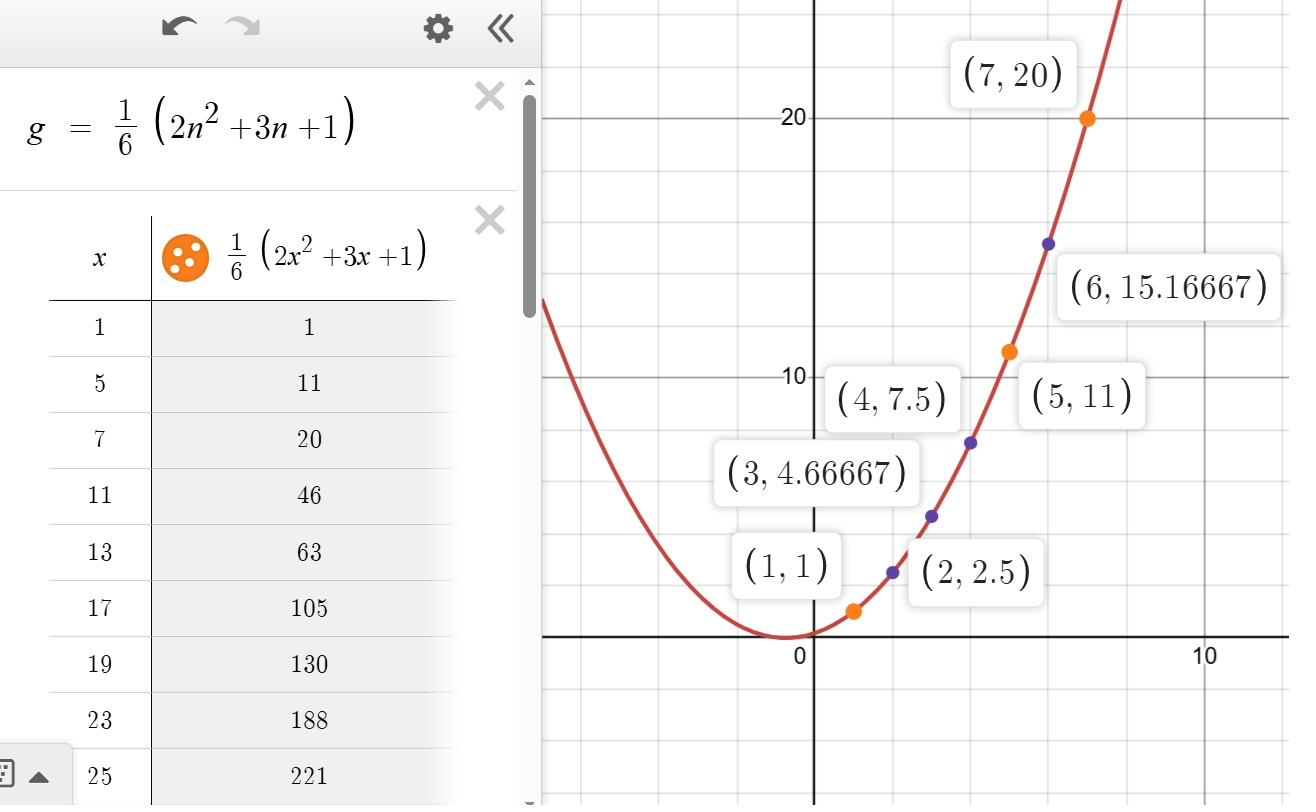
\includegraphics[width=0.85\textwidth]{bilder/Quadratische_kurve1}
  \caption{The quadratic curve $k(n) = \tfrac{1}{6}(2n^2+3n+1)$ as a continuous
    parabola with its numerical value table. The orange dots mark the
    integer values at $n \equiv 1,5 \pmod{6}$; the purple dots
    correspond to the non-integer intermediate values. The growth of the sequence
    is already clearly visible from the first values $(1,\,1),\,(5,\,11),\,(7,\,20)$.}
  \label{fig:quadratische_kurve}
\end{figure}

\section{Differences: Minor and Major Steps}

\begin{table}[htbp]
\centering
\caption{Differences of the integer values}
\begin{tabular}{*{15}{c}}
\toprule
$\Delta k$ & 10 & 9 & 26 & 17 & 42 & 25 & 58 & 33 & 74 & 41 & 90 & 49 & 106 & 57 \\
\bottomrule
\end{tabular}
\end{table}

\section{Generating Function of the Sequence \texorpdfstring{$k(n)$}{k(n)}}

We consider the sequence of quadratic means


\[
  k(n) \coloneqq \frac{1}{n}\sum_{j=1}^{n} j^{2}
  = \frac{2n^{2} + 3n + 1}{6}, \qquad n \ge 1.
\]



For this sequence we define the ordinary generating function


\[
  K(x) \coloneqq \sum_{n=1}^{\infty} k(n)\,x^{n}.
\]



\begin{theorem}
The generating function of $k(n)$ is a rational function of the form


\[
  K(x)
  = \frac{1}{6}\left(
      2\,\frac{x(1+x)}{(1-x)^{3}}
      + 3\,\frac{x}{(1-x)^{2}}
      + \frac{x}{1-x}
    \right),
\]


that is,


\[
  K(x) = \sum_{n=1}^{\infty} \frac{2n^{2} + 3n + 1}{6}\,x^{n}.
\]


\end{theorem}

\begin{proof}
From the explicit representation


\[
  k(n) = \frac{2n^{2} + 3n + 1}{6}
\]


it follows that


\[
  K(x)
  = \sum_{n=1}^{\infty} k(n)\,x^{n}
  = \frac{1}{6}\sum_{n=1}^{\infty} (2n^{2} + 3n + 1)\,x^{n}.
\]


We decompose the sum into three standard series:


\[
  K(x)
  = \frac{1}{6}\left(
      2\sum_{n=1}^{\infty} n^{2}x^{n}
      + 3\sum_{n=1}^{\infty} n x^{n}
      + \sum_{n=1}^{\infty} x^{n}
    \right).
\]


The closed forms for these series are well known:


\[
  \sum_{n=1}^{\infty} x^{n} = \frac{x}{1-x}, \qquad
  \sum_{n=1}^{\infty} n x^{n} = \frac{x}{(1-x)^{2}}, \qquad
  \sum_{n=1}^{\infty} n^{2} x^{n} = \frac{x(1+x)}{(1-x)^{3}},
\]


where all series converge for $|x|<1$. Substituting yields


\[
  K(x)
  = \frac{1}{6}\left(
      2\,\frac{x(1+x)}{(1-x)^{3}}
      + 3\,\frac{x}{(1-x)^{2}}
      + \frac{x}{1-x}
    \right).
\]


This establishes the stated representation.
\end{proof}

\begin{remark}
The rational structure of $K(x)$ reflects the fact that $k(n)$ is described
by a polynomial of degree two in $n$. From the representation of $K(x)$ one
can, for instance, obtain a linear recurrence for $k(n)$ by considering the
common denominator $(1-x)^{3}$ and comparing coefficients of $x^{n}$.

At the same time, $K(x)$ arises as a linear combination of the generating
functions of $n$, $n^{2}$, and the constant sequence~$1$. Thus $k(n)$ fits
naturally into the context of simple linear and quadratic sequences. The
generating function provides an alternative, analytic perspective on the same
structure that is already visible discretely in the congruence-theoretic
considerations (Theorem~\ref{satz:primzahlen}).
\end{remark}

\subsection{Linear Recurrence from the Generating Function}

From the rational representation of $K(x)$ a linear recurrence for the
sequence $k(n)$ can be derived immediately. To this end we write


\[
  K(x) = \sum_{n=1}^{\infty} k(n)\,x^{n}
\]


and consider the factor $(1-x)^{3}$:


\[
  (1-x)^{3} K(x)
  = (1 - 3x + 3x^{2} - x^{3}) \sum_{n=1}^{\infty} k(n)\,x^{n}.
\]


Expanding the product and comparing the coefficients of $x^{n}$ for
sufficiently large $n$ yields


\[
  k(n) - 3k(n-1) + 3k(n-2) - k(n-3) = 0 \qquad \text{for } n \ge 4.
\]


Thus the linear recurrence


\[
  k(n) = 3k(n-1) - 3k(n-2) + k(n-3), \qquad n \ge 4,
\]


holds, with initial values


\[
  k(1) = 1,\quad k(2) = \frac{5}{2},\quad k(3) = \frac{14}{3}.
\]



\begin{remark}
The recurrence reflects the fact that $k(n)$ is given by a polynomial of
degree two in $n$: a sequence described by a polynomial of degree $d$
always satisfies a linear recurrence of constant order $d+1$ with constant
coefficients. In the present case $d=2$, and the order of the recurrence
is~$3$.

Together with the explicit representation


\[
  k(n) = \frac{2n^{2} + 3n + 1}{6}
\]


and the congruence-theoretic condition for integer values
(Section~\ref{sec:arithmetik}), the generating function thus provides an
alternative, analytic perspective on the same structure. It connects the
discrete summation formula, the quadratic form of $k(n)$, and the
arithmetic patterns of the sequence within a common framework.
\end{remark}
